\documentclass[12pt]{article}

\usepackage{answers}
\usepackage{setspace}
\usepackage{graphicx}
\usepackage{enumitem}
\usepackage{multicol}
\usepackage{mathrsfs}
\usepackage[margin=1in]{geometry} 
\usepackage{amsmath,amsthm,amssymb,mathtools}
\usepackage{titlesec}

\newcommand\numberthis{\addtocounter{equation}{1}\tag{\theequation}}

\titleformat{\section}[runin]{\normalfont\Large\bfseries}{\thesection}{1em}{}
\titleformat{\subsection}[runin]{\normalfont\large\bfseries}{\thesubsection}{1em}{}

\def\tf{\textbf}
\def\tt{\textit}
\def\mc{\ensuremath\mathcal}
\def\mf{\ensuremath\mathbf}
\def\mt{\ensuremath\mathit}
\def\mb{\ensuremath\mathbb}
\def\td{\ensuremath\tilde}
\def\N{\ensuremath\mb{N}}
\def\Z{\ensuremath\mb{Z}}
\def\C{\ensuremath\mb{C}}
\def\R{\ensuremath\mb{R}}
\def\S{\ensuremath\mb{S}}
\def\Ber{\ensuremath\mf{Ber}}
\def\det{\ensuremath\mf{det}}
\def\sigm{\ensuremath\mf{sigm}}
\def\diag{\ensuremath\mf{diag}}
\def\dom{\ensuremath\mf{dom}}
\def\cond{\ensuremath\mf{cond}}
\def\sign{\ensuremath\mf{sign}}
\def\bd{\ensuremath\mf{bd}}
\def\arg{\ensuremath\mf{arg}}
\def\rto{\ensuremath\rightarrow\ }
\def\Rto{\ensuremath\Rightarrow\ }
\def\lto{\ensuremath\leftarrow\ }
\def\Lto{\ensuremath\Leftarrow\ }
\def\xrto{\ensuremath\xrightarrow}
\def\xRto{\ensuremath\xRightarrow}
\def\xlto{\ensuremath\xleftarrow}
\def\xLto{\ensuremath\xLeftarrow}
\def\rvec{\ensuremath\overrightarrow}
\def\lvec{\ensuremath\overleftarrow}

\providecommand\P[1]{}
\renewcommand\P[1]{\mb{P}\{#1\}}
\providecommand\E[1]{}
\renewcommand\E[1]{\mb{E}[#1]}
\providecommand\Var[1]{}
\renewcommand\Var[1]{\mf{Var}(#1)}
\providecommand\p[2]{}
\renewcommand\p[2]{\frac{\partial #1}{\partial #2}}
\providecommand\pp[2]{}
\renewcommand\pp[2]{\frac{\partial^2 #1}{\partial #2^2}}
\providecommand\ps[3]{}
\renewcommand\ps[3]{\frac{\partial^2 #1}{\partial #2\partial #3}}
\providecommand\d[2]{}
\renewcommand\d[2]{\frac{d #1}{d #2}}

\DeclareMathOperator{\sech}{sech}
\DeclareMathOperator{\csch}{csch}
    
\begin{document}
    
\title{Geometry and Complex Arithmetic - Notes}
\author{Dhruv Kohli}
\maketitle
\begin{itemize}
    \item Geometric rules for complex numbers: addition $\equiv$ vector addition, multiplication $=$ $R\angle \theta r\angle\phi$ $=$ $Rr\angle (\theta+\phi)$.
    \item Cardano argument: $ax^2+bx+c=0$ has roots $x = \frac{-b\pm\sqrt{b^2-4ac}}{2a}$. If $b^2<4ac$ then it leads to impossible numbers so discard such solutions. In the particular case of quadratic equations, this is perfectly fine to do. $ax^2=-bx-c$, LHS is a parabola and RHS is a line. When $b^2<4ac$ then line does not intersect the parabola so there will be no solution (with any physical meaning).
    \item Bombelli argument: Consider $x^3 = 3px+2q$. LHS is a cubic and RHS is a line. There will always be atleast one point of intersection. General solution is of form $x = (q+\sqrt{q^2-p^3})^{1/3} + (q-\sqrt{q^2-p^3})^{1/3}$. $q^2<p^3$ leads to impossible numbers (according to Cardano), but we can't discard solution (because there will be atleast one intersection). Bombelli wild thought: If $q^2<p^3$ then take $\sqrt{q^2-p^3}=i\sqrt{p^3-q^2}$ (ofcourse he worked out a specific example).
    \item Representation of complex numbers: Cartesian: $z=x+iy$, unique representation. Polar: $z=r\angle\theta$, non-unique representation, $r=|z|, \theta = \arg z$.
    \item Symbolic rules: addition: $(a+ib)+(\td{a}+i\td{b}) = (a+\td{a})+i(b+\td{b})$. multiplication: $(a+ib)(\td{a}+i\td{b}) = (a\td{a}-b\td{b}) +i (a\td{b}+\td{a}b)$.
    \item Geometric rules of addition and multiplication are same as symbolic rules. Equivalence of addition is easy to show. Geometric rule of multiplication means rotation of plane by $\theta$ and expansion by $R$. Symbolic rule of multiplication means $i^2=-1$ and brackets can be multiplied out $A(B+C)=AB+AC$. $G \implies S$: $i\cdot i = $ Rotate $i$ by $\pi/2$ which makes it $-1$ and parallelograms are preserved by rotation and expansion (see figure). $S \implies G$: If $z=x+iy$ then according to $S$, $iz = -y+ix$ which is nothing but rotation of $z$ by $\pi/2$. In general, $(a+ib)z = az + b(iz) = \text{exp}^{n}_{a}(z) + \text{exp}^{n}_{a}(\text{rot}^{n}_{\theta}(z))$ [Proved later].
    \begin{figure}[h!]
        \centering
        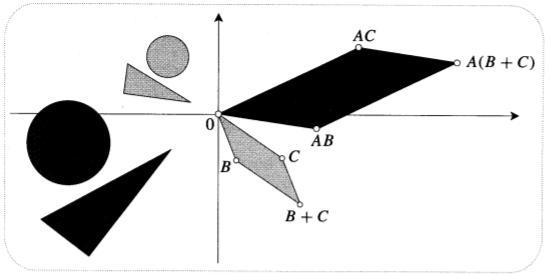
\includegraphics[scale=0.7]{fig_1}
        \label{f1}
    \end{figure}
    \item Euler's formula: $e^{i\theta} = \cos\theta + i\sin\theta$. Moving particle argument: $z(t) = e^{it}$, $z(0) = 1+0i$. $v(t) = \frac{dz(t)}{dt} = ie^{it}=iz(t)$. After $t=\theta$, since, $|z(t)|=1$ (particle traversing on circle of radius $1$) and $|v(t)|=1$ (speed of particle is $1$). Therefore, distance travelled is $\theta$. So, $z(\theta) = \cos\theta+i\sin\theta$; Power series argument: Use power series of $\cos \theta$, $\sin \theta$ and $e^{i\theta}$.
    \item $\sin\theta = (e^{i\theta}-e^{-i\theta})/2i$ and $\cos\theta = (e^{i\theta}-e^{-i\theta})/2$.
    \item Application of complex numbers is trigonometry: 
    
    \begin{align*}
        \cos(\theta+\phi) + i\sin(\theta+\phi) &= e^{i(\theta+\phi)}\\
        &= e^{i\theta}e^{i\phi}\\
        &= (\cos\theta+i\sin\theta)(\cos\phi+i\sin\phi)\\
        &= (\cos\theta\cos\phi - \sin\theta\sin\phi) + i(\cos\theta\sin\phi + \sin\theta\cos\phi)
    \end{align*}
    \begin{align*}
        \cos 4\theta+i\sin 4\theta &= e^{i4\theta}\\
        &= (e^{i\theta})^{4}\\
        &= (\cos\theta+i\sin\theta)^4\\
    \end{align*}
    \begin{align*}
        \cos^4\theta &= ((e^{i\theta}+e^{-i\theta})/2)^4 = \ldots
    \end{align*}
    \begin{align*}
        T &= \tan\theta\\
        z &= 1+iT\\
        \tan\theta &= \frac{\mf{Im} z}{\mf{Re} z}\\
        \tan 3\theta &= \frac{\mf{Im}(z^3)}{\mf{Re}(z^3)}
    \end{align*}
    \item Application of complex numbers in geometry: Consider a quadrilateral, draw squares on the edges of the quadrilateral outwards, the lines joining the centres of the opposite squares are equal in length and perpendicular to each other. Using complex numbers to show this: Let $2a,2b,2c,2d$ be the complex number representing consecutive edges of the quadrilateral. Let the one of the vertex be origin (from where edge $2a$ originates and edge $2d$ ends). Then $2a+2b+2c+2d = 0$. Let centres of the squares be $p,q,r,s$. Then,
    \begin{align*}
        p &= a+ia\\
        q &= 2a+b+ib\\
        r &= 2a+2b+c+ic\\
        s &= 2a+2b+2c+d+id\\
        A &= r-p\\
        &= a-ia +2b+c+ic\\
        B &= s-q\\
        &= b -ib + 2c+d+id\\
        A-iB &= a-ia+2b+c+ic-(ib + b +2ic + id -d)\\
        &= a+b+c+d -i(a+b+c+d)\\
        &= 0
    \end{align*}
    \begin{figure}[h!]
        \centering
        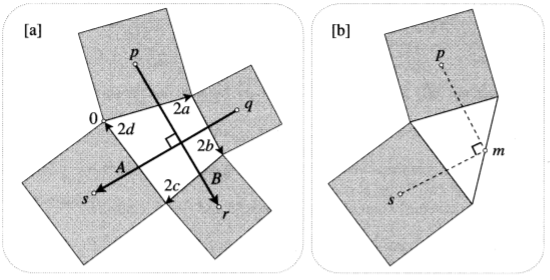
\includegraphics[scale=0.85]{fig_2}
        \label{f2}
    \end{figure}
    \item A naive approach to solve above problem is as follows. Translation transformation is given by,
    \begin{align*}
        T_v(z) = z+v    
    \end{align*}
    Rotational transformation about a point $a$ is given by,
    \begin{align*}
        R^{\theta}_{a}(z) &= T_a \circ R^{\theta}_{0} \circ T_{-a}(z)\\
        &= e^{i\theta}(z-a)+a    
    \end{align*}

    Note that,

    \begin{align*}
        R^{\theta_1}_{a} \circ R^{\theta_2}_{b}(z) &= R^{\theta_1}_{a}(e^{i\theta_2}(z-b)+b)\\
        &= e^{i(\theta_1+\theta_2)}z + e^{i\theta_1}b(1-e^{i\theta_2}) + a(1-e^{i\theta_1})\\
        &= z+c \qquad \text{when } \theta_1+\theta_2=2\pi
    \end{align*}

    In general, \tt{when $M = R^{\theta_1}_{a_1} \circ R^{\theta_2}_{a_2} \ldots \circ R^{\theta_n}_{a_n}$ and $\sum_{i=1}^{n}\theta_i = 2\pi$, then $M = T_{v}$}.\\~\\
    
    Coming back to the problem, we will show that $pm = sm$ and $pm \perp sm$.  Consider $M = R^{\pi}_{m}\circ R^{\pi/2}_{p}\circ R^{\pi/2}_{s}$. Using the above result, $M = T_{v}$. To find $v$ we just need to find image of one point. Note that $M(k) = k$ so, $v = 0$. So, $R^{\pi/2}_{p}\circ R^{\pi/2}_{s} = R^{-\pi}_{m}$. Consider $s' = R^{-\pi}_{m}(s)$. Then $s' = R^{\pi/2}_{p}\circ R^{\pi/2}_{s}(s) = R^{\pi/2}_{p}(s)$. Therefore, $ps = ps'$. $\Delta sps'$ is then an isosceles triangle with $\angle sps' = \pi/2$. This proves the result.

    \begin{figure}[h!]
        \centering
        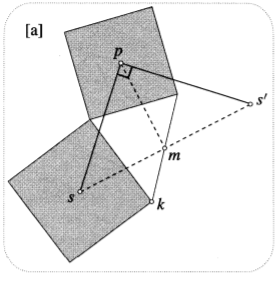
\includegraphics[scale=0.85]{fig_3}
        \label{f3}
    \end{figure}

    \item Cotes results: An approach to write $x^n-1$ as product of linear and quadratic terms with real coeddicients. Note that, $x^n-1 = \prod_{i=1}^{n}(x-a_i)$ where $a_i$ are roots of $x^n=1$. Since complex roots of such equation must occur in conjugates, if $a_i \in \C$, then $\exists j \neq i$ s.t. $a_j = \bar{a_i}$ so that $(x-a_i)(x-a_j)$ is a quadratic with real coefficients. Cotes followed this problem in a remarkable way. Consider a regular $n$-gon $C_1,C_2,\ldots,C_n$ s.t. these points lie on a circle of unit radius. Let $P$ be a point on the line passing from $0$ through $C_1$ at a distance $x>1$ from $0$. Then, $U_n(x) = x^n-1 = \prod_{i=1}^{n}PC_i$. Note that, in the figure, $C_2 = \bar{C_3}$ and $PC_2 = PC_3$ so that $PC_2PC_3$ is a quadratic in $x$.

    \begin{figure}[h!]
        \centering
        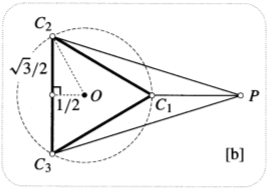
\includegraphics[scale=0.85]{fig_4}
        \label{f4}
    \end{figure}

    \item Vectorial operations: $a.b = |a||b|\cos\theta$ and $a\times b = |a||b|\sin\theta$ (defined differently in general). Cross product represents the signed area of a parallelogram. Now, consider, $a = r_1e^{i\theta_1}$ and $b= r_2e^{i\theta_2}$, where $\theta_1-\theta_2 = \theta$ then,
    
    \begin{align*}
        a\bar{b} &= r_1r_2 e^{i(\theta_1-\theta_2)}\\
        &= r_1r_2e^{i\theta}\\
        &= r_1r_2(\cos\theta+i\sin\theta)\\
        &= a.b + ia\times b
    \end{align*}
    \item Area of polygon whose vertices are represented by $a,b,c,d$ is given by,

    \begin{align*}
        &\frac{1}{2}(a\times b + b\times c + c\times d + d\times a)\\
        &= \frac{1}{2}\mf{Im}(a\bar{b}+b\bar{c}+c\bar{d}+d\bar{a})
    \end{align*}

    Since the each of the term represents a signed area, the case when $0$ is outside the polygon, is implicitly handled.

    \begin{figure}[h!]
        \centering
        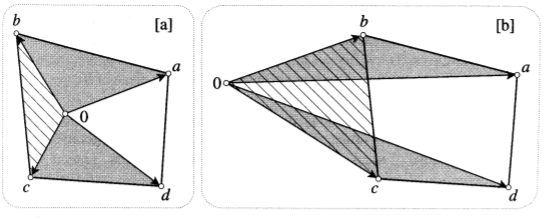
\includegraphics[scale=0.85]{fig_5}
        \label{f5}
    \end{figure}

    \item $M$=motion $=$ mapping/transformation of a plane to itself that preserves distance i.e. $d(A,B) = d(f(A),f(B))$.
    \item $F\cong F'$ if there exists $M$ s.t. $F'=M(F)$.
    \item Geometric properties of a figure are those which are unaltered by set of all possible motions.
    \item Geometric equalty can in general be denoted by an equivalence relation between figures. Keeping this general definition of geometric equality in mind, the motion can itself be defined in general as a family $G$ of transformations which forms a group.
    \item Note that distance preserving transformations do form a group (identity preserved distance, composition of distance preserving transformation is another distance preserving transformation, inverse of a distance preserving transformation preserves distance $c=f(a),d=f(b), d(f^{-1}(c),f^{-1}(d)) = d(a,b) = d(f(a),f(b)) = d(c,d)$) and thus constitute a special family of transformations.
    \item Klein's idea: Take a group of transformations $G$ and define the corresponsing geometry as the study of invariants of $G$.
    \item \tt{A motion is uniquely determined by its effect on any trianle (i.e. on any three non-collinear points)}.
    \item Note that a point $P$ is uniquely determined by its distances from vertices of a triangle. Given distances from two vertices, there are only two choices of location for $P$. Distance from third vertex finalizes which among the two choices should be the exact location of $P$.

    \begin{figure}[h!]
        \centering
        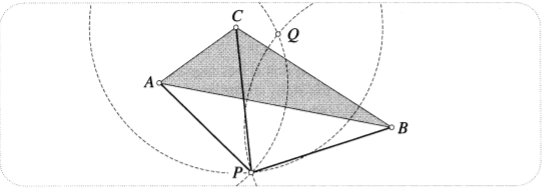
\includegraphics[scale=0.85]{fig_6}
        \label{f6}
    \end{figure}

    \item Now, given that we know the image of a triangle. Let $P$ be a general point. Since motion is distance preserving, the distance of image of $P$ will be at same distances from images of $A,B,C$ as the distance of $P$ from $A,B,C$. Thus we know we know where each point on the plane will map.

    \begin{figure}[h!]
        \centering
        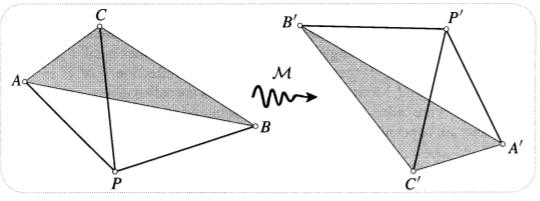
\includegraphics[scale=0.85]{fig_7}
        \label{f7}
    \end{figure}

    \item Classifying motions in two types: Suppose a motion sends $A$ to $A'$ and $B$ to $B'$. Still, the motion is not determined. Now, motion will send a third point $C$ to one of the two choices, $C'$ and its reflection $\td{C}$ in the line through $A'$ and $B'$. Thus there are two motions that map $A,B$ to $A',B'$: $\mc{M}$ sends $C$ to $C'$ and $\td{\mc{M}}$ sends $C$ to $\td{C}$. The two motions differ in the sense that $\mc{M}$ preserves sense of the angle $\theta$ which $\td{\mc{M}}$ reverses it. $\mc{M}$ preserves all angles while $\td{\mc{M}}$ reverse all angles. Motion that preserve angles are called \tt{direct} and those that reverse angles are called \tt{opposite}. Thus rotations and translations are direct, while reflections are opposite.

    \begin{figure}[h!]
        \centering
        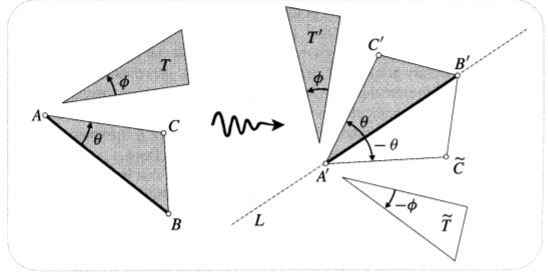
\includegraphics[scale=0.85]{fig_8}
        \label{f8}
    \end{figure}

    \item \tt{There is exactly one direct motion $\mc{M}$ (and exactly one opposite motion $\td{\mc{M}}$) that maps a given line-segment $AB$ to another line segment $A'B'$ of equal length. Furthermore, $\td{\mc{M}} = \mc{M}$ followed by reflection in the line $A'B'$.}

    \item \tt{Every direct motion is a rotation, or else (exceptionally) a translation}. See figure for proof. Based on the rotational transformation that we did before, we have, \tt{Every direct motion can be expresed as a complex function of the form $\mc{M}(z) = e^{i\theta}z+v$}.

    \begin{figure}[h!]
        \centering
        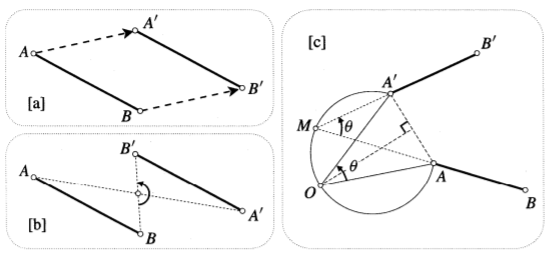
\includegraphics[scale=0.85]{fig_9}
        \label{f9}
    \end{figure}

    \item Set of direction motions form a subgroup of the group of motions while set of opposite motions do not.

    \item \tt{Every direct motion is the composition of two reflections}. Therefore, every opposite motion is a composition of three reflections. This is three reflections theorem.

    \item \tt{If $L_1$ and $L_2$ intersect at $O$, and the angle from $L_1$ to $L_2$ is $\phi$, then, $\mc{R}_{L_2} \circ \mc{R}_{L_1}$ is a rotation of $2\phi$ about $O$}. \tt{If $L_1$ and $L_2$ are parallel, and $V$ is the perpendicular connectng vector from $L_1$ to $L_2$, then $\mc{R}_{L_2} \circ \mc{R}_{L_1}$ is a translation of $2V$}.

    \begin{figure}[h!]
        \centering
        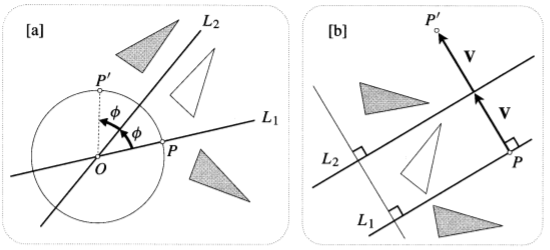
\includegraphics[scale=0.85]{fig_10}
        \label{f10}
    \end{figure}

    \item Rotation of $\theta$ can be represented as $\mc{R}_{L_2}\circ\mc{R}_{L_1}$, where $L_1,L_2$ is any pair of lines that pass through the centre of the rotation and that contain an angle $\theta/2$.
    \item A translation of $T$ corresponds to any pair of parallel lines separated by $T/2$. To see the combined effect of two rotation, see the figure.

    \begin{figure}[h!]
        \centering
        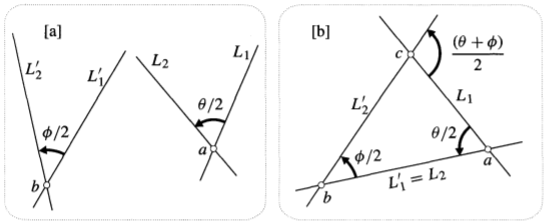
\includegraphics[scale=0.85]{fig_11}
        \label{f11}
    \end{figure}

    \item \tt{A similarlity $\mc{S}$ is a mappig of the plane to itself that preserves ratios of distances}. A similarity $\mc{S}$ expands every distance by same (non-zero) factor $r$ known as \tt{expansion} of $\mc{S}$. Set of all similarities $\mc{S}^{r}$ form a group.
    \item \tt{Euclidean geometry is the study of those properties of geometric figures that are invariant under the group of similarities}.
    \item Note that motions are just $\mc{S}^{1}$. The group of motions is a subgroup of the group of similarities.
    \item Central dilation $D_{o}^{r}$ is an example of $S^{r}$ that leaves $o$ fixed and radially stretches each segment $oA$ by $r$. If this is followed by (or preceded by) a rotation $R_{o}^{\theta}$ with same centre, then we get dilative rotation $D_{o}^{r,\theta} \equiv R_{o}^{\theta} \circ D_{o}^{r} = D_{o}^{r} \circ R_{o}^{\theta}$.
    \item Taking $o$ to be the origin of $\C$, dilative rotation $D_{o}^{r,\theta}$ corresponds to multiplication by $re^{i\theta}$. Conversely, \tt{the rule of complex multiplication may be viewed as a consequence of the behaviour of dilative rotations}.
    \item Note that $D_{o}^{R,\phi} \circ D_{o}^{r,\theta} = D_{o}^{Rr,\phi+\theta}$. So, if complex numbers are viewed as translations then composition yields complex addition and when they are viewed as dilative rotations then composition yields multiplications.
    \item Note that if $p$ is an arbitrary point then $\mc{M} \equiv \mc{S}^r \circ D^{1/r}_{p}$ is a motion. Thus any similarity is the composition of a dilation and a motion: $\mc{S}^r = \mc{M} \circ D^{r}_{p}$.
    \item If $\mc{M}$ preserves angles then so is $\mc{S}^r$ and we get direct similarity. If $\mc{M}$ reverses angles then so will $\mc{S}^r$ and we get opposite similarity.
    \item \tt{Every direct similarity is a dilative rotation or (exceptionally) a translation}. \tt{Every direct similarity \mc{S}^r can be expressed as a complex function of the form $S^{r}(z) = re^{i\theta}z + v$}.
\end{itemize}
\end{document}
            